\documentclass[11pt,a4paper]{article}
\usepackage[T1]{fontenc}
\usepackage{lmodern,microtype}
\usepackage[margin=27mm,headheight=14pt]{geometry}
\usepackage{amsmath,amssymb,amsthm,booktabs,array,graphicx}
\usepackage[authoryear,round]{natbib}
\usepackage{caption,subcaption,fancyhdr,enumitem,xcolor}
\usepackage[colorlinks=true,linkcolor=blue!45!black,citecolor=blue!45!black,urlcolor=blue!45!black]{hyperref}
\usepackage[section]{placeins}
\setlength{\parskip}{2pt}
\setlength{\emergencystretch}{1em}
\setlength{\parindent}{1.2em}
\captionsetup{font=small,labelfont=bf}
\pagestyle{fancy}\fancyhf{}
\fancyhead[L]{\small Cheap Search, Costly Holds}\fancyhead[R]{\small Gupta}
\fancyfoot[C]{\thepage}\renewcommand{\headrulewidth}{.3pt}
\newtheorem{theorem}{Theorem}
\newtheorem{proposition}[theorem]{Proposition}
\newtheorem{corollary}[theorem]{Corollary}
\newcommand{\E}{\mathbb E}
\newcommand{\Pp}{\mathbb P}
\newcommand{\support}{\operatorname{supp}}
\title{\vspace{-12mm}\textbf{Cheap Search, Costly Holds:\\Reservation Synchronization in Agentic Markets}}
\author{Shivam Gupta\\\small Independent Researcher, India\\\small\href{mailto:shivam1720406@gmail.com}{shivam1720406@gmail.com}}
\date{16 October 2026}
\begin{document}
\maketitle
\begin{abstract}
Shopping agents can reserve several alternatives while completing only one purchase. What happens when reducing the cost of search expands these temporary claims on capacity? We distinguish the number of reservation attempts, their duration, and their joint release. First, an exact finite-market construction gives two systems with the same one-supplier request, acceptance, and holding-time process but a transaction-success ratio that grows linearly with market size. Independently expiring holds and a common release decision therefore cannot be compared using marginal capacity telemetry alone. Second, in an independent-availability economic model, all symmetric equilibria can be enumerated through adjacent-action indifference equations. When holding duration grows as the search breadth to a positive power, vanishing search cost drives equilibrium completion probability to zero; bounded holding duration gives a positive limit. A scalar family of linear programs supplies global planner bounds, and a capacity-time toll supports a planner optimum. In a declared numerical example, reducing per-attempt cost from 0.03 to 0.01 increases equilibrium breadth from 12 to 32 and reduces completion probability from 0.718 to 0.432, while planner welfare increases. Exact finite-state calculations, rational-arithmetic checks, and event-driven experiments separate the economic mechanism from the approximation used to calculate it. The results motivate mandate-linked reservation accounting and duration-sensitive controls for agentic commerce, without treating simulated parameters as estimates of marketplace behavior.
\end{abstract}
\noindent\textbf{Keywords:} agentic commerce; search costs; temporary reservations; congestion externalities; market design.\\
\textbf{JEL:} C72, D83, L86.\\
\textbf{Research materials:} \url{https://github.com/shi1720/cheap-search-costly-holds}.

\section{Introduction}
A shopping assistant can compare many suppliers at low computational cost. If comparing an alternative merely retrieves a quote, additional search principally consumes information-processing resources. If comparison requires an exclusive reservation, the assistant also removes capacity from other buyers. The distinction is economically consequential even when the assistant purchases at most one item and releases every unused reservation correctly.

This paper asks three questions. Can supplier-level reservation telemetry establish whether a market is serving buyers effectively? Can an innovation that lowers the private cost of search reduce the probability of completing a transaction? Which object should a platform price or constrain if it wants to preserve the benefits of delegated search?

These questions concern an identifiable interface in commerce systems. Shopify's versioned draft-order documentation distinguishes ordinary draft creation from explicit inventory reservation and exposes an automatic-restocking time \citep{shopify}. Its checkout documentation also specifies that inventory is held at payment submission rather than during ordinary browsing \citep{checkout}. These distinctions rule out a blanket claim that browsing agents necessarily reserve stock. Our analysis applies when an authorized workflow actually takes exclusive, temporary capacity claims. The capacity can represent a reusable reservation-stage slot; post-commitment occupation is introduced separately. It is not a model of indefinitely depleted physical inventory.

Existing economic and operations research already establishes that multiple applications, no-shows, redundant requests, and congestion can create externalities. Relabeling these phenomena as agent behavior would add little. The present contribution is narrower: it separates the scale and timing of temporary claims, derives an exact comparison that preserves a supplier's complete pre-commitment capacity process, and characterizes a cheap-search limit in which expanding deliberation time undermines successful trade. The economic model and the finite reservation system are kept distinct throughout.

The first result is finite and exact. There are $M$ identical suppliers, one temporary slot at each, and buyers arrive at rate $\lambda M$. Every buyer requests all $M$ slots. Compare a common exponential release clock for all accepted holds with independent exponential clocks of the same mean at each hold. In either system, a supplier sees an $M/M/1/1$ reservation process with offered rate $\lambda M$ and mean holding time $\tau$. Nevertheless, the probability that an arriving buyer obtains any hold is $1/(1+\lambda M\tau)$ under common release and $1/(1+\lambda\tau)$ under independent release. Their ratio grows proportionally to $M$. The observation restriction matters: these identical processes describe reservation requests, occupancy, and releases, excluding final purchase labels and cross-supplier linkage. Completed-order records would reveal the difference.

The second result concerns incentives under a specified independent-availability benchmark. An arriving buyer chooses reservation breadth $k$, pays search cost $ck$, and values obtaining at least one hold at $v$. The mean duration of each accepted hold is $\tau_k$, so its capacity-time demand is $h_k=k\tau_k$. The equilibrium distribution of $k$ determines slot availability. Under $\tau_k\sim a k^\beta$ with $\beta>0$, cheaper attempts generate more outstanding capacity-time than completed transactions: equilibrium breadth grows as $c^{-1/(\beta+1)}$, while completion probability falls as $c^{\beta/(\beta+1)}$. A constant duration produces a positive limit instead. The claim is consequently about the joint evolution of search cost and holding time, not an inevitable cost of automation.

The third contribution is computational. We enumerate every symmetric equilibrium for a finite breadth menu, globally bound planner welfare through interval linear programs, and derive the occupancy toll supporting a planner optimum. Finite-state and event-driven calculations then test when the independent-availability benchmark describes an actual collection of slots. They also expose its failure for market-wide, synchronized holds. The code, experimental specification, run-level results, and figure scripts are public.

\section{Relationship to existing research}
\paragraph{Search and multiple applications.}
\citet{albrecht} analyze equilibrium directed search when workers submit multiple applications, including endogenous application choices. Their model already contains coordination failures among applicants and vacancies. Their finite-market correction is particularly relevant: failure probabilities at different vacancies need not factorize \citep{correction}. We use the same elementary union-of-successes expression only inside an explicitly independent benchmark. Our finite construction concerns repeated, exclusive occupancy and common release clocks, rather than wage posting or a one-period offer allocation. We do not claim that multiple-search inefficiency or endogenous search breadth is new.

\paragraph{Reservations and strategic multi-listing.}
\citet{alexandrov} explain why capacity-constrained services may offer reservations despite no-show costs. \citet{chen} study strategic multi-listing across differentiated service queues and demonstrate that throughput and welfare comparisons can differ. Their cancel-upon-entry and cancel-upon-service mechanisms allocate service through the earliest available or completed copy. Our model instead has immediate loss rather than waiting, temporary occupation of every available alternative during a decision interval, and a holding duration indexed by the attempted breadth. The distinguishing claims are the matched reservation-process comparison and the cheap-search scaling result, not the desirability of pricing congestion.

\paragraph{Loss networks, redundancy, and dependence.}
Loss networks supply the established capacity-accounting framework \citep{kelly}; batch admission control studies partial acceptance of arriving groups \citep{ormeci}. In our finite system, accepted holds have a common mandate clock, which requires retaining group sizes in the state. Redundancy research already shows that dependence between copies can alter system performance \citep{anton}. Here, successful reservation of at least one alternative is the economic outcome, and a release ends a temporary claim rather than completing the fastest service copy. More broadly, \citet{agrawal} study the consequences of ignoring dependence in stochastic optimization. Our linear gap is a constructive dynamic comparison, not a new general claim that marginals fail to determine joint outcomes.

\paragraph{Congestion pricing.}
\citet{naor} provides the classic private-versus-social queueing comparison and toll remedy. We use the same economic logic. The contribution is a particular occupancy price, a complete equilibrium enumeration for the declared reservation model, and an explicit global objective bound. The paper does not introduce Pigouvian pricing, a new general loss-network approximation, or a new mechanism for enforcing identity across platforms.

\section{Temporary capacity claims}
\subsection{Finite reservation system}
There are $M$ exchangeable suppliers with one reusable reservation slot each. Buyers arrive as a Poisson process of rate $\lambda M$, where $\lambda>0$ is demand per slot per unit time. An arriving buyer chooses $k\leq M$ distinct suppliers uniformly without replacement. It immediately obtains a hold at each selected supplier that is idle; busy suppliers reject the request. No rejected request waits or retries within that mandate.

If at least one hold is obtained, the mandate completes one eventual transaction worth $v$ by assumption, without later execution failure. Success is recorded at admission; the study does not model product selection by a language model or subsequent payment execution. All other claims are unused alternatives. The baseline isolates reservation-stage capacity: every accepted slot is released after its holding interval, and the final transaction consumes no further capacity from this particular pool. This is the $s=0$ case. Section~\ref{sec:extension} adds mean post-commitment occupation $s$ at the selected slot. The baseline therefore measures temporary reservation congestion, not every physical resource used in production or consumption.

Under \emph{common release}, all holds accepted for a mandate use one common lifetime, independent across mandates and independent of availability at admission. Its mean is $\tau_k>0$. We examine both exponential and deterministic lifetimes. Under the \emph{independent-release control}, each accepted hold instead has its own independent exponential lifetime with the same mean. A buyer chooses at most one accepted alternative for eventual completion; unused alternatives expire. Different release clocks change neither the one-hold lifetime distribution nor the number of attempts. They change the dependence of releases across suppliers.

Let $q$ denote the stationary idle probability of a randomly chosen supplier, and let $P_M(k)$ be the probability an arriving buyer obtains at least one hold. For a fixed $k$, expected accepted holds per arrival are exactly $kq$, by uniform sampling and Poisson-arrival sampling \citep{wolff}. Conservation of occupied slot-time gives
\begin{equation}
 1-q=\lambda kq\tau_k,\qquad
 q=\frac{1}{1+\lambda k\tau_k}.\label{eq:exactq}
\end{equation}
No independence between suppliers is needed for this marginal identity. The lifetime assumption must exclude a dependence of its mean on the number accepted; otherwise $kq\tau_k$ need not be the expected total hold-time.

By contrast, $P_M(k)$ depends on the joint idle pattern. If $F$ suppliers are idle just before arrival,
\begin{equation}
 P_M(k)=\E\left[1-\frac{\binom{M-F}{k}}{\binom{M}{k}}\right],\label{eq:hypergeom}
\end{equation}
where a binomial coefficient with insufficient elements is zero. The function of $F$ is not determined by $\E F=Mq$. This is the precise location of the independence approximation used later.

\begin{figure}[t]
\centering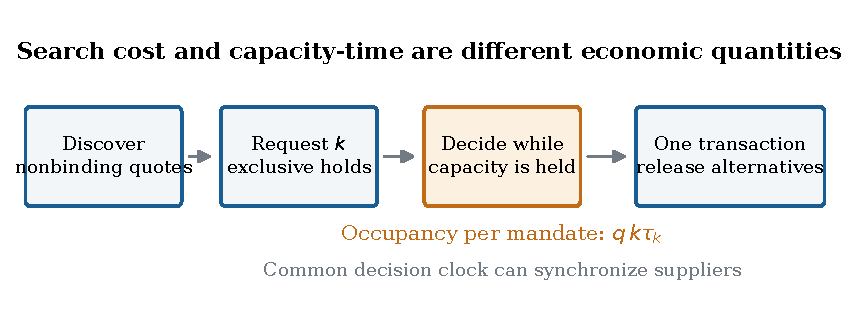
\includegraphics[width=\linewidth]{../figures/mechanism.pdf}
\caption{The reservation boundary. Search that only obtains quotes does not create the modeled capacity claim. Binding holds occupy capacity until release; one successful mandate generates at most one transaction. Common release links several suppliers to one decision clock. The economic benchmark assumes independent availability at admission, whereas the finite system explicitly retains joint occupancy.}
\label{fig:mechanism}
\end{figure}

\subsection{Identical supplier processes, different transaction success}
\begin{theorem}[A matched reservation-process gap]\label{thm:gap}
Let $k=M$, start from an empty system, set $s=0$, and take exponential lifetimes of mean $\tau>0$. Under common release and independent release, the reservation process at any single supplier has the same law: offered arrivals are Poisson of rate $\lambda M$, idle arrivals are accepted, and an accepted hold has an exponential lifetime of mean $\tau$. Nevertheless,
\begin{equation}
 P_M^{\mathrm{common}}(M)=\frac{1}{1+\lambda M\tau},\qquad
 P_M^{\mathrm{independent}}(M)=\frac{1}{1+\lambda\tau}.\label{eq:gap}
\end{equation}
Thus the independent-to-common success ratio is
$(1+\lambda M\tau)/(1+\lambda\tau)$, even though both systems have $q=1/(1+\lambda M\tau)$.
\end{theorem}
\begin{proof}
With common release, the first arrival to an empty system takes all slots and holds them for a common exponential interval. All subsequent arrivals are rejected until that interval ends. The system alternates between an empty interval of mean $1/(\lambda M)$ and an all-occupied interval of mean $\tau$. Its idle-time fraction is the first expression in~\eqref{eq:gap}, and Poisson arrivals see that fraction.

With independent release, every arrival leaves all $M$ slots occupied: it fills precisely the slots that became idle since the preceding arrival. Immediately after an arrival, the $M$ residual lifetimes are independent exponentials of mean $\tau$, including those of surviving holds by memorylessness. Let $T$ be the next interarrival time, exponential of rate $\lambda M$. The next buyer fails exactly when no slot releases during $T$. Its failure probability is
\[
 \E[e^{-MT/\tau}]=\frac{\lambda M}{\lambda M+M/\tau}
 =\frac{\lambda\tau}{1+\lambda\tau}.
\]
Finally, each supplier separately receives every Poisson arrival and has the same exponential accepted-hold law in both systems. These facts identify its complete reservation-state process and establish the matched marginal law.
\end{proof}

The theorem restricts observation to \emph{one-supplier pre-commitment capacity telemetry}: requests, acceptances, occupancy, and releases. It excludes completed-order labels, other suppliers' states, and joined mandate records. It does not say a merchant cannot measure its sales. It says that equal request volume, acceptance probability, and holding-time distributions do not certify an equal market-level flow of distinct successful mandates.

The independent-release system is also not a collection of independently occupied suppliers: shared arrival times still correlate their states. Substituting $1-(1-q)^M$ gives a third quantity. At $\lambda\tau=1$ this approximation tends to $1-e^{-1}$; the independent-release result is $1/2$, while common release tends to zero. An approximation can therefore miss both the quantitative level and the order of magnitude.

\section{Search incentives under independent availability}
\subsection{A declared economic benchmark}
To isolate incentives at small breadth relative to the market, assume that an arriving mandate sees each of its attempted suppliers idle independently with probability $q$. This is a model assumption, not a consequence of~\eqref{eq:exactq}. It gives
\begin{equation}
 P_k(q)=1-(1-q)^k,\quad P_0(q)=0.\label{eq:ind}
\end{equation}
Buyers choose $k\in\{0,1,\ldots,K\}$, where $k=0$ permits abstention. A distribution $p=(p_0,\ldots,p_K)$ specifies the population's choices. Let $h_0=0$, $h_k=k\tau_k$, $H(p)=\sum_k p_kh_k$, and $\bar k=\sum_kp_kk$. For the baseline,
\begin{equation}
 q(p)=\frac{1}{1+\lambda H(p)},\qquad
 U_k(q)=vP_k(q)-ck.\label{eq:utility}
\end{equation}
The value $v>0$ is net of exogenous purchase price and production cost. Cost $c>0$ is a real resource or effort cost per attempt, rather than a transfer. The buyer is risk neutral, does not observe current occupancy before choosing $k$, and takes aggregate $q$ as given. It does not pay directly for tying up other buyers' capacity. In particular, there is no private disutility from delay in the baseline; its relaxation is consequential, as discussed below.

A symmetric equilibrium is a distribution $p$ supported on maximizers of $U_k(q(p))$. Welfare per supplier per time is
\begin{equation}
 W(p)=\lambda\sum_kp_kU_k(q(p)).\label{eq:welfare}
\end{equation}
This is a partial-equilibrium demand-side model. Supplier prices, entry, investment, buyer budgets, and bargaining are held fixed. It is not a welfare theorem for a complete retail economy.

\subsection{Enumerating all symmetric equilibria}
\begin{proposition}[Adjacent support and exhaustive enumeration]\label{prop:enum}
Suppose $h_k$ is strictly increasing for $k\geq0$. Every finite-menu symmetric equilibrium has either one action or two adjacent actions in its support. Pure action $k$ is an equilibrium exactly when $U_k(q_k)$ is maximal, where $q_k=(1+\lambda h_k)^{-1}$. An interior mixture of $k$ and $k+1$ must satisfy
\begin{equation}
 vq(1-q)^k=c,\qquad
 x=\frac{q^{-1}-1-\lambda h_k}{\lambda(h_{k+1}-h_k)}\in(0,1),\label{eq:mix}
\end{equation}
with $p_{k+1}=x$. For $k\geq1$, the indifference equation has at most two roots in $(0,1)$, one on each side of $1/(k+1)$; for $k=0$ it has at most one. Testing these roots and all pure actions enumerates every symmetric equilibrium.
\end{proposition}
\begin{proof}
At fixed $0<q<1$, successive utility increments are
$U_{k+1}-U_k=vq(1-q)^k-c$, strictly decreasing in $k$. The maximizing actions are consequently a singleton or two adjacent integers. An adjacent indifference is globally optimal by this decreasing-increment property. Substituting $H=(1-x)h_k+xh_{k+1}$ into~\eqref{eq:utility} gives~\eqref{eq:mix}. The derivative of $q(1-q)^k$ has the sign of $1-(k+1)q$, proving the root count. At $q=1$, the unique best action for $c<v$ is $1$; all abstention has $q=1$ and cannot be an equilibrium in that case. The remaining boundary and equality cases are checked directly among pure actions.
\end{proof}

The finite-menu equilibrium correspondence is nonempty by applying a fixed-point theorem to the best-response correspondence on the probability simplex: utilities are continuous and the best-response sets are nonempty, compact, and convex after mixing. Uniqueness is not asserted. For example, $\lambda=0.001$, $\tau_k=0.001+(k-1)$ for $k\geq1$, $v=1$, and $c=0.001$ admit pure breadths $1$ and $2$, together with an interior mixture. The solver therefore retains every admissible root instead of selecting the outcome of a particular adjustment dynamic.

\subsection{A cheap-search limit}
\begin{theorem}[Growing holding duration]\label{thm:cheap}
Consider the independent-availability benchmark with unbounded integer breadth, $s=0$, fixed $\lambda,v>0$, and $\tau_k\sim a k^\beta$ for $a,\beta>0$. Along any sequence of symmetric equilibria as $c\downarrow0$, let $\kappa$ be the lower support action; a pure equilibrium uses its single action. Then $\kappa\to\infty$, adjacent mixing is asymptotically immaterial, and
\begin{align}
 \kappa &\sim \left(\frac{v}{\lambda a c}\right)^{1/(\beta+1)},\label{eq:kscale}\\
 P^{\mathrm{eq}} &\sim (\lambda a)^{-1/(\beta+1)}
                   (c/v)^{\beta/(\beta+1)}\longrightarrow0,\label{eq:pscale}\\
 W^{\mathrm{eq}} &\sim \frac{\lambda v}{2}
                    (P^{\mathrm{eq}})^2\longrightarrow0.\label{eq:wscale}
\end{align}
The same statements apply to increasing finite caps whenever the equilibrium support is interior to the cap eventually.
\end{theorem}
\begin{proof}
If equilibrium support stayed bounded along a subsequence, $H$ would stay bounded and availability would stay strictly positive. The marginal gain from another attempt at the largest support action would then be bounded away from zero, contradicting $c\to0$. Proposition~\ref{prop:enum} implies adjacent support, so $H\sim a\kappa^{\beta+1}$ and
$q\sim(\lambda a\kappa^{\beta+1})^{-1}$. Hence $\kappa q\to0$.

For a pure interior equilibrium the two adjacent-increment inequalities give
$vq(1-q)^\kappa\leq c\leq vq(1-q)^{\kappa-1}$; at a mixture the lower expression equals $c$. Both imply $c\sim vq$, yielding~\eqref{eq:kscale}. Expanding $1-(1-q)^\kappa\sim\kappa q$ gives~\eqref{eq:pscale}.

For the welfare equivalent, write $z=\kappa q\to0$. Uniformly over adjacent support,
$P=z-z^2/2+o(z^2)+O(q)$, but the $O(q)$ change in first-order success is canceled by the corresponding first-order change in search cost when the support is mixed. More explicitly, put $k=\kappa+J$, where $J\in\{0,1\}$. Then
\[
 \E P_k(q)=\E[k]q-\tfrac12\E[k(k-1)]q^2+O((\kappa q)^3),
\]
and the equilibrium marginal-cost inequalities imply
$c/v=q-\kappa q^2+O(\kappa^2q^3)+O(q^2)$.
Subtracting $(c/v)\E k$ leaves $z^2/2+o(z^2)$, because $\kappa\to\infty$ and $z\to0$. Multiplication by $\lambda v$ proves~\eqref{eq:wscale}.
\end{proof}

The mechanism is an externality, not a mistaken maximization by the buyer. At fixed $q$, extra attempts offer a positive chance of obtaining capacity. In the population, the same choices expand $k\tau_k$, reduce $q$, and erode other mandates' success. The limit does not require an adverse effect of breadth on the value of the selected product.

\begin{proposition}[Bounded duration is a substantive countercase]\label{prop:constant}
Under the same assumptions except $\tau_k\to\tau_\infty\in(0,\infty)$, set $b=(\lambda\tau_\infty)^{-1}$. Along interior equilibrium sequences as $c\downarrow0$,
\[
 P^{\mathrm{eq}}\to1-e^{-b}>0,\quad
 c\bar k\to vb e^{-b},\quad
 W^{\mathrm{eq}}\to\lambda v[1-(1+b)e^{-b}]>0.
\]
\end{proposition}
\begin{proof}
The bounded-support contradiction still gives $\kappa\to\infty$. Now $q\sim b/\kappa$, so $\kappa q\to b$ and $(1-q)^\kappa\to e^{-b}$. The adjacent marginal conditions give $c\sim vb e^{-b}/\kappa$, establishing each limit.
\end{proof}

The two collapse results have different quantifiers. Theorem~\ref{thm:cheap} is a cheap-search limit \emph{inside} the independent benchmark, with duration growing in breadth. Theorem~\ref{thm:gap} is an exact finite-system result with market-wide breadth and constant duration. Neither licenses exchanging the limits of market size, breadth, and holding time.

\section{A globally bounded planner and an occupancy toll}\label{sec:planner}
A planner chooses the population distribution $p$. Fixing $q$ makes its problem linear. For the baseline, feasible distributions satisfy
\begin{equation}
 \sum_kp_k=1,\quad p_k\geq0,\quad
 \lambda q\sum_kp_kh_k=1-q,\label{eq:lp}
\end{equation}
with objective $\lambda\sum_kp_k[vP_k(q)-ck]$. The feasible range is $q\in[(1+\lambda h_K)^{-1},1]$. A fixed-$q$ optimum exists with at most two positive probabilities by the standard basic-solution structure of a linear program with two equality constraints. These actions need not be adjacent: planner sparsity and equilibrium concavity are different statements.

A dense scalar grid alone does not certify a global optimum. For $q\in[l,u]$, monotonicity of $P_k$ bounds the reward by its value at $u$. We relax capacity balance to
\begin{equation}
 \lambda l\sum_kp_kh_k\leq1-l,\qquad
 \lambda u\sum_kp_kh_k\geq1-u.\label{eq:bound}
\end{equation}
Maximizing the upper reward over these constraints yields an upper bound on every planner value in that interval. Feasible fixed-$q$ solutions and pure policies supply lower bounds. Bisecting the interval with the largest upper bound produces a reported global gap. This is an analytic bounding construction evaluated with floating-point LPs; it is not an exact-arithmetic certificate for arbitrary real-valued inputs. The numerical experiments require a gap below $10^{-7}$ and separately report the solver's residuals where applicable.

\begin{proposition}[Supporting the planner with capacity-time pricing]\label{prop:toll}
Let $p^*$ globally maximize~\eqref{eq:welfare}, with finite $K$, and write $q^*=q(p^*)$. Define
\begin{equation}
 B=\lambda v\sum_kp_k^*k(1-q^*)^{k-1},\quad
 D=1+\lambda H(p^*),\quad \pi^*=B/D,\label{eq:toll}
\end{equation}
where the $k=0$ term is zero. Charging $\pi^*$ per unit of occupied slot-time supports $p^*$ as a price-taking equilibrium. The expected charge for action $k$ is $\pi^*q^*h_k$. Fee revenue is treated as a transfer when evaluating social welfare.
\end{proposition}
\begin{proof}
For any simplex direction $d$ at $p^*$,
$\partial q/\partial p[d]=-\lambda q^*\sum_kd_kh_k/D$.
Differentiating welfare gives
\[
 \partial W[d]=\lambda\sum_kd_k\{vP_k(q^*)-ck-\pi^*q^*h_k\}.
\]
At a global optimum every feasible direction moving mass from a supported action to any action has nonpositive derivative. Thus each supported action maximizes the expression in braces, which is precisely private expected payoff at the announced toll and availability. This establishes support as an equilibrium, without asserting uniqueness or convergence of a price-adjustment rule.
\end{proof}

A fee for an accepted request that is fully refunded on cancellation can leave temporary occupancy unpriced. Conversely, an undiscounted per-attempt charge need not reflect duration. The relevant benchmark here is payment for occupied capacity-time, including unused alternatives, rather than payment for the single final purchase alone. The price $\pi^*$ depends on demand, values, and the induced distribution. It is a supporting price for the declared model, not a revenue-maximizing merchant tariff.

\subsection{Post-commitment capacity and private waiting costs}\label{sec:extension}
Suppose the chosen alternative occupies its slot for additional mean time $s\geq0$ after deliberation; all unchosen alternatives release at the end of the holding interval. Under independent availability, balance becomes
\begin{equation}
 F(q,p)=q+\lambda\sum_kp_k[qh_k+sP_k(q)]-1=0.\label{eq:service}
\end{equation}
It has a unique solution because $F$ is strictly increasing in $q$. At fixed $q$, it remains an affine constraint in $p$. Interval bounds use $F(l,p)\leq0\leq F(u,p)$ and upper reward at $u$. Equilibrium enumeration still uses the same private indifference roots; mixture probabilities follow from~\eqref{eq:service} instead of~\eqref{eq:mix}.

The supporting occupancy price becomes $\pi^*=B/D$ with
$D=1+\lambda\sum_kp_k[h_k+sP'_k(q)]$. Its expected charge is
$\pi^*[qh_k+sP_k(q)]$. The derivative proof is unchanged. This extension prices both temporary alternatives and the selected slot's subsequent use. It does not make the exact full-fanout formulas in Theorem~\ref{thm:gap} valid for $s>0$.

Private waiting cost can remove the cheap-search singularity. For example, let $\tau_k=t_0+a(k-1)$ for $k\geq1$ and subtract a direct delay cost $d\tau_k$ from private utility. Among positive actions, the marginal cost of breadth becomes $c+da$. For any $d>0$, this floor remains as $c\to0$, preventing the unbounded interior breadth used in Theorem~\ref{thm:cheap}. Likewise, reducing holding time jointly with search cost can change the conclusion. An empirical assessment must measure both margins; cheaper tokens alone do not identify a market-level welfare effect.

\section{Computational evidence}\label{sec:experiments}
\subsection{Design and verification}
All numerical parameters are declared scenarios in consistent, normalized time and value units. They are not fitted to a marketplace. The baseline sets $\lambda=v=1$, $\tau_k=0.2+0.05(k-1)$ for positive $k$, and permits abstention. The central menu has $K=128$ and costs $0.03$, $0.01$, and $0.003$. Parameter exploration preceded a frozen experimental specification and a 10,000-arrival pilot. This is not a preregistered empirical study. The saved plan and source hashes identify the specification used for the main run.

Verification has three layers. First, the common-exponential finite system is solved by a continuous-time Markov chain (CTMC). Its state $n_j$ counts active mandates holding $j$ slots. Admission transitions have hypergeometric probabilities from~\eqref{eq:hypergeom}; departures remove one group at rate $n_j/\tau_k$. A separate labeled-slot implementation builds the chain using bitmask groups, solves stationarity by rational Gaussian elimination, and agrees for all 15 cases with $1\leq k\leq M\leq5$. These are independently constructed state representations, not two calls to the same transition builder.

Second, 231 finite CTMC cases cover every breadth for $M=2,\ldots,12$ and $\lambda\in\{0.2,1,3\}$ at $\tau=1$. Third, a physical-slot event simulator retains actual occupied suppliers and timed releases, rather than CTMC group-count states. It checks that every release concerns an occupied slot and that capacity is never over-allocated. Its validation cases vary $M\in\{128,512,2048\}$, $k\in\{1,3,12,32\}$, and common exponential versus common deterministic holding times. Each case uses 24 independent seeds, 20,000 warm-up arrivals, and 100,000 counted arrivals. Separate full-fanout cases use $M\in\{8,32,128,512\}$, both release controls, and 200,000 counted arrivals per seed. A final set uses $s=0.5$, $M=2048$, and $k\in\{3,12,32\}$.

Run-level means and two-sided Student-$t$ 95\% intervals describe Monte Carlo precision across independent runs. They are not confidence intervals for real demand parameters, and we make no population hypothesis tests or field-effect claims. The suite additionally verifies best-response inequalities in 216 parameter configurations and checks planner bounds against feasible portfolios. Full logs include every run rather than selecting favorable seeds.

\subsection{Search cost and the planner frontier}
\begin{table}[t]
\centering\small
\caption{Independent-availability benchmark. All symmetric equilibria are enumerated; each central case has one. Welfare is net real surplus per supplier-time, with $\lambda=v=1$. Planner objective upper gaps are at most $10^{-7}$.}
\label{tab:central}
\begin{tabular}{rrrrrrr}\toprule
&\multicolumn{3}{c}{Decentralized equilibrium}&\multicolumn{3}{c}{Planner}\\
\cmidrule(lr){2-4}\cmidrule(lr){5-7}
Cost $c$ & Mean $k$ & Success & Welfare & Mean $k$ & Success & Welfare\\\midrule
\csname @@input\endcsname central_rows.tex
\bottomrule\end{tabular}
\end{table}

Reducing $c$ from $0.03$ to $0.01$ expands equilibrium breadth from $12$ to $32$, while the completion probability falls from $0.7176$ to $0.4324$ (Table~\ref{tab:central}). The lower cost is a real technological improvement at fixed behavior. Its equilibrium effect is adverse because mean duration rises from $0.75$ to $1.75$, and attempted capacity-time per mandate rises from $9$ to $56$. Availability falls from $0.1$ to $1/57$. Equilibrium welfare falls from $0.3576$ to $0.1124$.

The planner benefits from the cheaper technology: its optimal breadth remains $2$ in these two scenarios, and welfare rises from $0.8289$ to $0.8689$. At $c=0.003$, the equilibrium mixes adjacent breadths near $70$, while the planner selects breadth $3$. Supporting occupancy prices are $0.4444$, $0.4444$, and $0.3543$ respectively; the saved payoff checks show no profitable deviation at the displayed pure planner solutions to floating-point tolerance. These comparisons are benchmark optima, not optimized policies for the finite simulator.

\begin{figure}[t]
\centering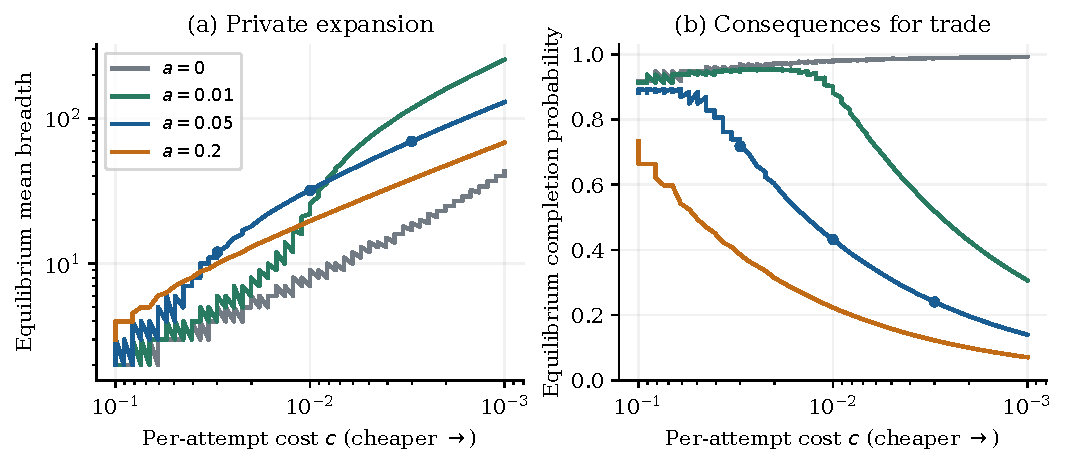
\includegraphics[width=\linewidth]{../figures/economics.pdf}
\caption{Equilibrium response to cheaper attempts under independent availability. Curves enumerate equilibria with $K=512$, $\lambda=v=1$, and $\tau_k=0.2+a(k-1)$. The displayed cost range avoids a binding cap. A constant duration ($a=0$) is the substantive negative control; growing duration changes the direction of the low-cost response. Dots identify the central declared scenarios.}
\label{fig:econ}
\end{figure}

\subsection{Exact dependence and finite-market approximation}
\begin{figure}[t]
\centering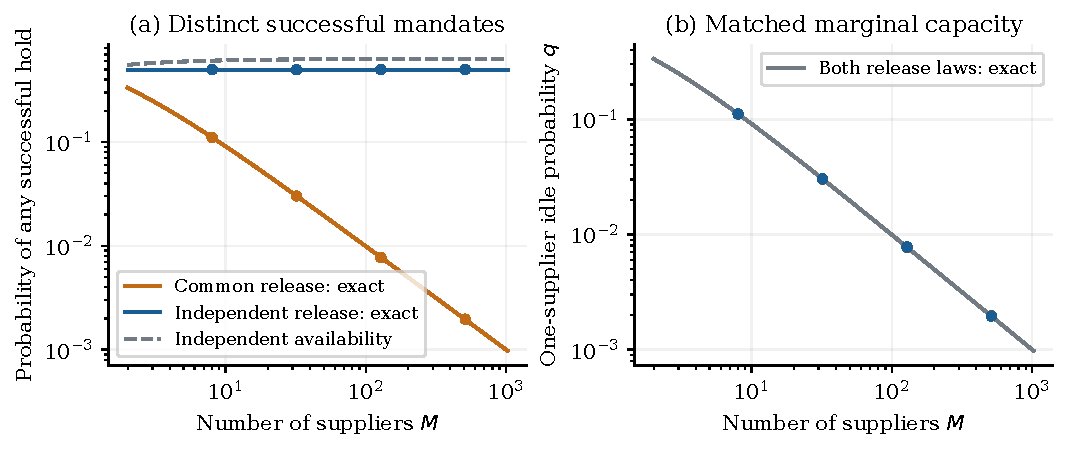
\includegraphics[width=\linewidth]{../figures/full_fanout.pdf}
\caption{Full-market breadth at $\lambda=\tau=1$. Exact success is $1/(1+M)$ with common release and $1/2$ with independent release. Both have the same one-supplier idle probability $1/(1+M)$. Points and 95\% run-level intervals are event simulations with 24 seeds. The independently occupied-supplier formula is a separate approximation and is not the independent-release result.}
\label{fig:full}
\end{figure}

The finite-state calculations recover~\eqref{eq:exactq} and the closed-form endpoints. Figure~\ref{fig:full} illustrates the matched-process gap without using the independent-availability approximation. At $M=512$, the exact common-release success probability is $1/513$, while independent release gives $1/2$: a ratio of $256.5$. This is an extreme market-wide mandate, offered as a mechanism witness rather than a typical commerce workload.

At smaller breadth, finite correlations still matter. With $M=8$, $\lambda=\tau=1$, the CTMC yields success $0.54386$ for $k=2$ and $0.52073$ for $k=4$; independently occupied suppliers give $0.55556$ and $0.59040$. Correct marginal availability therefore does not make the union calculation exact, even well short of $k=M$.

\begin{table}[t]
\centering\small
\caption{Finite event validation for $M=2048$, common exponential release, and $\tau_k=0.2+0.05(k-1)$. Intervals quantify variation over 24 simulation seeds. The $s=0.5$ rows include additional occupation of the chosen slot.}
\label{tab:finite}
\begin{tabular}{rrrrr}\toprule
Post-use $s$ & Breadth $k$ & Benchmark success & Simulated success & 95\% interval\\\midrule
\csname @@input\endcsname finite_rows.tex
\bottomrule\end{tabular}
\end{table}

\begin{figure}[t]
\centering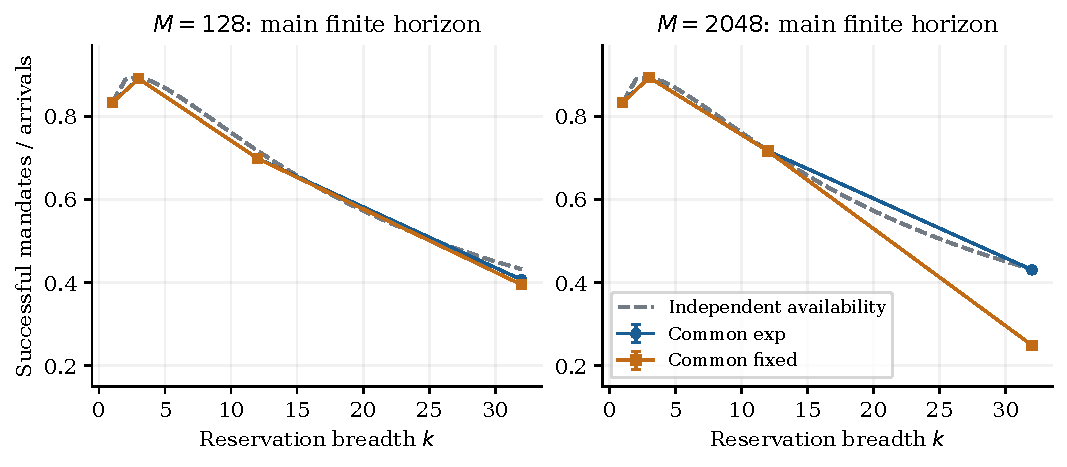
\includegraphics[width=\linewidth]{../figures/finite_validation.pdf}
\caption{Testing the independent-availability benchmark with distinct physical suppliers. Means and 95\% run-level intervals are shown for common exponential and common deterministic release. The benchmark is a reference line, not a finite-system theorem. Differences between market sizes and release distributions remain part of the reported evidence.}
\label{fig:finite}
\end{figure}

The main run contains 840 runs and 103.2 million counted arrivals (120 million including warm-up). Across the 231 finite CTMC cases, the largest stationarity residual is $1.4\times10^{-15}$ and the largest marginal-balance error is $4.4\times10^{-16}$. For common exponential release at $M=2048$, the largest absolute success discrepancy across the four tested breadths is 0.0016. The deterministic-release control is substantially different at breadth 32: the main-horizon success mean is 0.2494, compared with benchmark 0.4324, despite nearly unchanged mean availability. This motivates the separate horizon diagnostic below; these fixed-clock runs should not be interpreted as demonstrated stationary samples.


\subsubsection*{Diagnosing a fixed-clock transient}
The large deterministic-release discrepancy prompted a separate, explicitly exploratory horizon check, not a change to the frozen main specification. Six new seeds per cell use 500,000 counted arrivals after 20,000, 200,000, or 2,000,000 warm-up arrivals, at breadth 32 and $M\in\{512,2048\}$. The completion mean at $M=2048$ rises from 0.3391 at the shortest warm-up to 0.4310 at the longest (Figure~\ref{fig:horizon} and Table~\ref{tab:horizon}), close to the independent-availability benchmark 0.4324. The original 100,000-arrival observation window starts earlier and gives 0.2494. Thus the large original discrepancy should be attributed to a long startup/horizon effect in this experiment, rather than presented as an established stationary failure. At $M=512$, the longest-warm-up mean is 0.4269; residual finite-market dependence and remaining horizon sensitivity are not separated by this diagnostic. The diagnostic adds 36 runs and 18 million counted arrivals, retained separately from the main 840 runs.

\begin{figure}[t]
\centering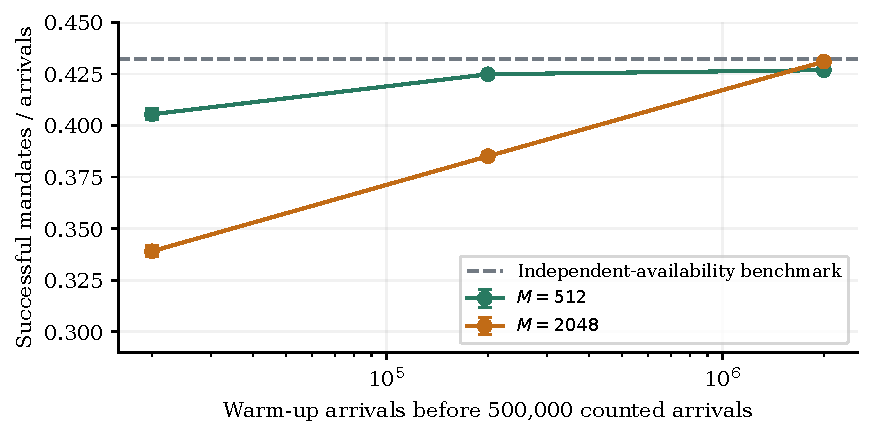
\includegraphics[width=.87\linewidth]{../figures/horizon_diagnostic.pdf}
\caption{Exploratory diagnosis of common deterministic release at breadth 32. Increasing the warm-up materially changes observed transaction success. Each point uses six fresh seeds and 500,000 counted arrivals; intervals describe run-level Monte Carlo variation. The long-horizon recovery prevents interpreting the main fixed-clock discrepancy as demonstrated stationary breakdown.}
\label{fig:horizon}
\end{figure}

\begin{table}[t]
\centering\small
\caption{Exploratory fixed-clock horizon check. The benchmark success is 0.4324 in every cell; these are finite observation windows, not proven stationary samples.}
\label{tab:horizon}
\begin{tabular}{rrrr}\toprule
Suppliers $M$ & Warm-up arrivals & Simulated success & 95\% interval\\\midrule
\csname @@input\endcsname horizon_rows.tex
\bottomrule\end{tabular}
\end{table}

For an additional asymptotic check, the artifact constructs exact interior pure equilibria at breadths from $16$ to $65{,}536$, with $\tau_k=0.05k^\beta$ and $\beta\in\{0.5,1,2\}$. It chooses cost between the two adjacent marginal benefits, rather than fitting a log-log regression. The stored ratios compare these values directly with~\eqref{eq:kscale}--\eqref{eq:pscale}. This is a deterministic check of the asymptotic algebra; it is not additional observed market evidence.

\section{Implications for market design and commercial systems}
The economic object is a temporary exclusive claim, not the label ``AI agent.'' A fast buyer making nonbinding requests can be beneficial. A slower buyer making very few binding claims can consume substantial capacity. Effective governance therefore requires at least three recorded quantities: attempted breadth, occupied capacity-time, and linkage of alternative holds to a single intended transaction. Aggregate order counts remain necessary for outcome measurement.

Theorem~\ref{thm:gap} identifies a reason to join reservations at mandate level. Identical one-supplier capacity processes can support very different counts of distinct successful buyers. A platform operating several reservation interfaces can record a pseudonymous transaction-scoped mandate identifier, creation and release times, accepted alternatives, and the one eventual conversion. These fields allow it to measure joint releases and unused hold-time directly. The analysis supplies no privacy guarantee for such identifiers; cross-platform linking requires its own consent, security, and governance design.

The supporting toll suggests a capacity-time budget or metered charge for holds, with an explicit maximum duration and a release obligation. A budget can be enforced by a broker within one mandate without banning broad nonbinding search. The mathematical price is a welfare benchmark for evaluating a policy, not evidence that a real market should immediately impose that fee. A cap can sacrifice valuable fallback options, and uniform fees can burden low-liquidity buyers. Extending the welfare model to values, budgets, and supplier heterogeneity is necessary before a distributional policy recommendation.

A commercial implementation could provide reservation telemetry, expiry enforcement, and a what-if simulator for booking platforms or agent gateways. Its customer proposition would be measurable improvements in completed distinct mandates per capacity-time, rather than raw request throughput. This paper supplies an auditable reference model and calculations; it does not estimate willingness to pay, market size, patentability, or commercial savings. The practical validation step would be to estimate the joint relationship between attempt breadth, holding time, and conversion from authorized operational logs, then evaluate a prospectively specified policy.

\section{Limitations and conclusion}
The results establish a particular failure mechanism and a computable economic response. They do not establish its current frequency. There are no observed buyer choices or fitted marketplace parameters in the computational study. The baseline ignores private discounting of delayed purchases, supplier differentiation, endogenous pricing, and permanent inventory depletion. Its clean cheap-search limit relies on growing holding duration and no compensating direct waiting cost. The exact synchronization comparison assumes full-market breadth, exponential lifetimes for both process laws, and no post-commitment occupation of this pool. These restrictions make the conclusions testable rather than universal.

The finite calculations also delimit the economic approximation. Marginal slot balance can be exact when a product of availability probabilities is inaccurate. The paper proves no general propagation-of-independence theorem as the number of suppliers grows. Large-market simulations at the declared small breadths provide numerical checks, while the full-fanout construction shows why they cannot justify an unrestricted extrapolation. Planner tolls support an optimum of the benchmark; they need not select it uniquely or implement a finite-market optimum.

Within these boundaries, three conclusions follow. Pre-commitment capacity telemetry does not determine distinct transaction success. Lower private search cost can reduce completion when the expansion of temporary capacity-time is sufficiently strong. A planner can preserve cheaper search while limiting its externality by valuing occupied capacity-time. Agentic markets should therefore distinguish discovering more alternatives from holding more of the market open while deciding.

\paragraph{Code and reproducibility.}
The public repository contains source, tests, a frozen experiment specification, provenance hashes, all run-level summaries, and scripts generating the manuscript's figures and tables. The main experimental results use synthetic events. The numerical planner bounds use SciPy/HiGHS floating-point optimization; the small labeled-state checks use exact rational arithmetic.

\paragraph{Competing interests.}
The author works in commercial AI product development and founded Siloed. The numerical study evaluates a declared reservation model rather than the performance of an employer's or client's product.

{\small\raggedright\setlength{\bibsep}{3pt}
\begin{thebibliography}{99}
\bibitem[Agrawal et~al.(2012)]{agrawal} Agrawal, S., Ding, Y., Saberi, A., and Ye, Y. (2012). Price of correlations in stochastic optimization. \emph{Operations Research}, 60(1), 150--162. \href{https://doi.org/10.1287/opre.1110.1011}{doi:10.1287/opre.1110.1011}.
\bibitem[Albrecht et~al.(2003)]{correction} Albrecht, J.~W., Gautier, P.~A., and Vroman, S.~B. (2003). Matching with multiple applications: The limiting case. Working paper, August. \url{https://units.georgetown.edu/economics/pdf/325.pdf}.
\bibitem[Albrecht et~al.(2006)]{albrecht} Albrecht, J., Gautier, P.~A., and Vroman, S. (2006). Equilibrium directed search with multiple applications. \emph{Review of Economic Studies}, 73(4), 869--891. \href{https://doi.org/10.1111/j.1467-937X.2006.00400.x}{doi:10.1111/j.1467-937X.2006.00400.x}.
\bibitem[Alexandrov and Lariviere(2012)]{alexandrov} Alexandrov, A., and Lariviere, M.~A. (2012). Are reservations recommended? \emph{Manufacturing \& Service Operations Management}, 14(2), 218--230. \href{https://doi.org/10.1287/msom.1110.0360}{doi:10.1287/msom.1110.0360}.
\bibitem[Anton et~al.(2021)]{anton} Anton, E., Ayesta, U., Jonckheere, M., and Verloop, I.~M. (2021). On the stability of redundancy models. \emph{Operations Research}, 69(5), 1540--1565. \href{https://doi.org/10.1287/opre.2020.2030}{doi:10.1287/opre.2020.2030}.
\bibitem[Chen et~al.(2024)]{chen} Chen, Z., Ding, Y., and Yang, L. (2024). Multi-listing for horizontally differentiated services. Working paper, June 18. \href{https://doi.org/10.2139/ssrn.4869846}{doi:10.2139/ssrn.4869846}. The June 2024 working-paper version is used here; the author-maintained research page lists a revised version as forthcoming in \emph{Operations Research} (2026).
\bibitem[Kelly(1991)]{kelly} Kelly, F.~P. (1991). Loss networks. \emph{Annals of Applied Probability}, 1(3), 319--378. \href{https://doi.org/10.1214/aoap/1177005872}{doi:10.1214/aoap/1177005872}.
\bibitem[Naor(1969)]{naor} Naor, P. (1969). The regulation of queue size by levying tolls. \emph{Econometrica}, 37(1), 15--24. \href{https://doi.org/10.2307/1909200}{doi:10.2307/1909200}.
\bibitem[\"Ormeci and Burnetas(2005)]{ormeci} \"Ormeci, E.~L., and Burnetas, A. (2005). Dynamic admission control for loss systems with batch arrivals. \emph{Advances in Applied Probability}, 37(4), 915--937. \href{https://doi.org/10.1239/aap/1134587747}{doi:10.1239/aap/1134587747}.
\bibitem[Shopify(2026a)]{shopify} Shopify (2026a). DraftOrder: GraphQL Admin API, version 2026-01. Accessed October 16, 2026. \url{https://shopify.dev/docs/api/admin-graphql/2026-01/objects/DraftOrder}.
\bibitem[Shopify(2026b)]{checkout} Shopify (2026b). Shopify checkout. Help Center. Accessed October 16, 2026. \url{https://help.shopify.com/en/manual/checkout-settings}.
\bibitem[Wolff(1982)]{wolff} Wolff, R.~W. (1982). Poisson arrivals see time averages. \emph{Operations Research}, 30(2), 223--231. \href{https://doi.org/10.1287/opre.30.2.223}{doi:10.1287/opre.30.2.223}.
\end{thebibliography}
}
\end{document}
